\chapter{Principaux points techniques}

%%%%%

\section{Architecture générale}

%%%%%%%%%%%%%%%%%%%%%%%%%%%
%% ARCHITECTURE GENERALE %%
%%%%%%%%%%%%%%%%%%%%%%%%%%%
Notre choix d'architecture se base sur la possiblité d'agir en 
multi-utilisateurs sur une machine, à travers une interface commune de 
communication vers le réseau.

Notre client peer-to-peer se décompose donc en un serveur local de fichiers 
(que nous désignerons dans ce rapport par le terme \textit{démon}), et un 
certain nombre de processus utilisateurs (que nous nommerons des 
\textit{clients}) connectés à cette interface réseau commune.
	

\subsection{Le client}
	La partie client de notre application sert à interagir avec 
l'utilisateur humain. Basiquement, l'utilisateur tape des commandes et le 
client lui renvoie un résultat généré par le démon.

La figure \ref{client} illustre l'architecture de notre client. Tout d'abord, 
le client se charge de créer un socket permettant de se connecter à son démon,
 avec l'IP et le port adéquats. Il crée ensuite un thread qui s'occupe de gérer
 l'envoi des commandes tapées par l'utilisateur. Ce thread crée lui-même un 
autre thread qui s'occupe d'afficher à l'écran les réponses aux commandes 
reçues du démon.

Le client s'occupe uniquement de renvoyer à l'utilisateur les réponses reçues
du démon. En conséquence, l'intégralité des requêtes utilisateurs ne sont pas 
gérées directement par la partie client de notre application, mais par le 
démon.
\begin{center}
\begin{figure}[htbp]
    \centering
    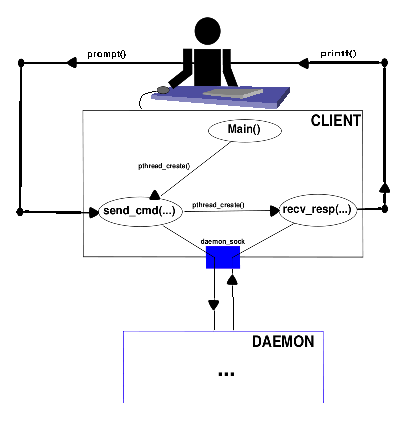
\includegraphics[scale=1.4]{archi_client.eps}
    \caption{Architecture du client}
    \label{client}
\end{figure}
\end{center}

	
\subsection{Le démon}

    Nous avons choisi de développer le serveur sous forme d'un démon.
S'éxécutant en arrière-plan, il peut à tout moment être contacté par un client
ou par un autre serveur utilisant le même protocole de communication.

    Dès qu'un client se connecte au démon, un thread est lancé et le gère
jusqu'à ce qu'il se déconnecte (cf. handle\_client () dans
\url{daemon/client_handler.c}). Il est ajouté à une liste doublement chaînée de
 clients connus, afin que l'application ait à tout moment une vision globale 
des clients qui lui sont affectés. 

\begin{lstlisting}
struct client {
    int                     socket;
    sem_t                   socket_lock;
    char                    *addr;
    pthread_t               thread_id;
    struct client_request   *requests;
    int                     nb_requests;
    sem_t                   req_lock;
    struct client           *next;
    struct client           *prev;
};
\end{lstlisting}

    On remarque ici qu'il est nécessaire d'utiliser des sémaphores afin d'éviter
les "situations de compétition". Un client pourrait en effet avoir besoin de
modifier son champ "requests", et a besoin d'être sûr qu'une seule modification
puisse être effectuée à la fois.

    Dès qu'un client envoie une commande au démon via sa socket, une nouvelle
"struct client\_request" est créée. Elle est ajoutée à la liste doublement
chaînée contenant toutes les requêtes actives pour le client. Un thread est
lancé pour traiter cette requête, et appelle la fonction correspondante dans
\url{daemon/client_requests/}.

\begin{lstlisting}
struct client_request {
    char                    *cmd;
    struct client           *client;
    void *                  (*handler) (void *);
    struct pool             *pool;
    phtread_t               tid;
    int                     assigned;
    struct client_request   *prev;
    struct client_request   *next;
};
\end{lstlisting}



%%%%%


\section{Gestion des threads}
\label{threads_by_pools}
Nos threads sont répartis en quatre "pools", plus un thread principal.


\subsection{Thread principal}
Le thread principal a deux sockets d'écoute, l'un destiné aux clients et
l'autre aux démons. Dès qu'il reçoit une requête de connexion sur l'un de
ses sockets, il redirige les démons vers le pool qui gère les démons et
les clients vers le pool qui gère les clients. Voir la figure \ref{interaction}.
\begin{center}
\begin{figure}[htbp]
    \centering
    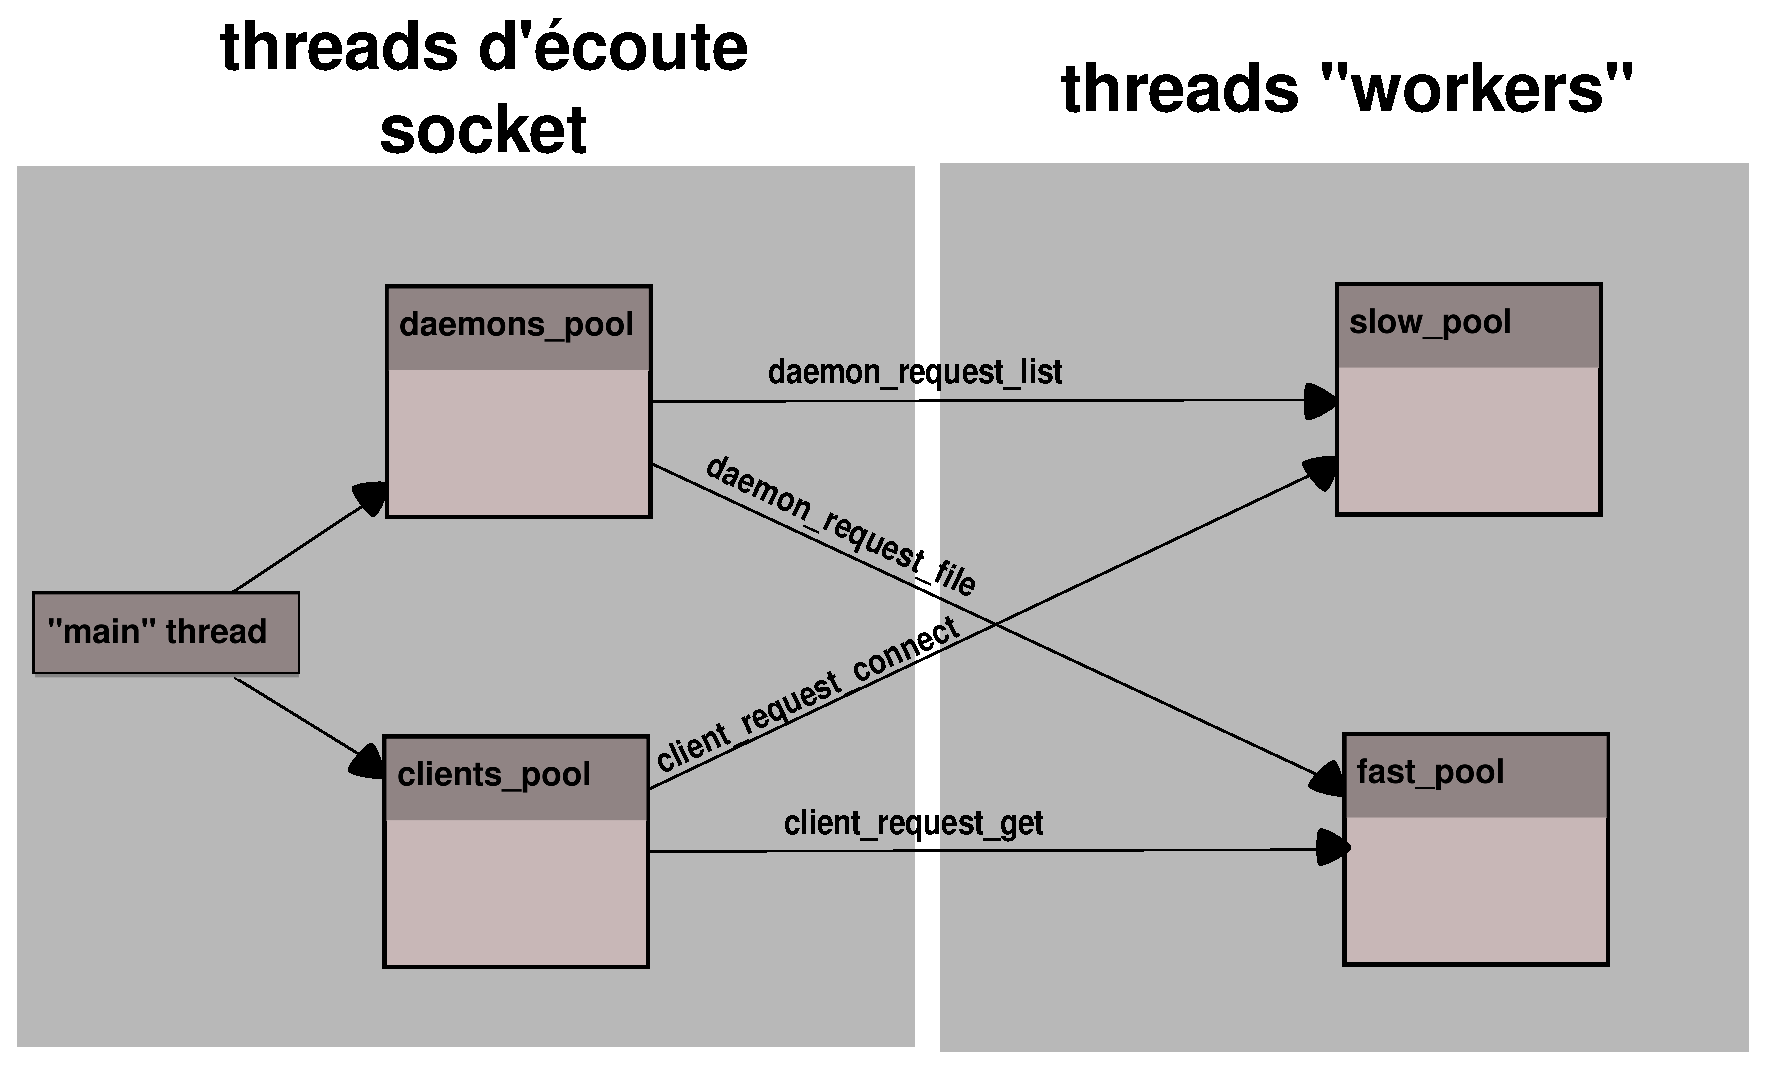
\includegraphics[scale=0.3]{pools_interacting.eps}
    \caption{Le thread principal et les 4 pools.}
    \label{interaction}
\end{figure}
\end{center}


\subsection{Pool de gestion des clients et des démons}
Nous avons donc deux pools de gestion : un pour les clients et un pour
les démons. Ils contiennent chacun un nombre de threads fixé par
l'utilisateur dans le fichier de configuration, sous les termes 
\verb$max_clients$ pour les clients et \verb$max_demons$ pour les démons.
Chaque thread est en charge d'un démon/client.

Ces deux pools sont des pools de threads dormants, qui ne se réveillent qu'à 
réception d'une requête. Ils envoient ensuite ces requêtes sur les deux autres
pools de threads et se rendorment.

\subsection{Le pool rapide et le pool lent}
Les deux autres pools gèrent donc les requêtes selon le temps qu'elles 
prennent : le premier pool gère les requêtes qui se font rapidement 
(par exemple \verb$help$) et le deuxième les requêtes plus complexes, qui 
prennent donc plus de temps comme \verb$list$ par exemple.

Cette séparation en deux pools est nécessaire car si nous n'avions qu'un seul 
pool de gestion des requêtes, il aurait vite été surchargé de requêtes lentes
donc les requêtes plus rapides ne pourraient pas s'exécuter (nombre de requêtes
simultanées maximal atteint). Dans notre configuration, les deux types de 
requêtes sont séparées, ainsi les deux ont accès au processeur à leur tour.

Ces deux pools contiennent autant de threads qu'il y a de coeurs sur la
machine. Ils peuvent s'envoyer des tâches à eux-mêmes ou à l'autre pool.\\

La figure \ref{fonctionnement} illustre le fonctionnement des pools de threads,
 avec des exemples de tâches externes et internes.

\begin{center}
\begin{figure}[htbp]
    \centering
    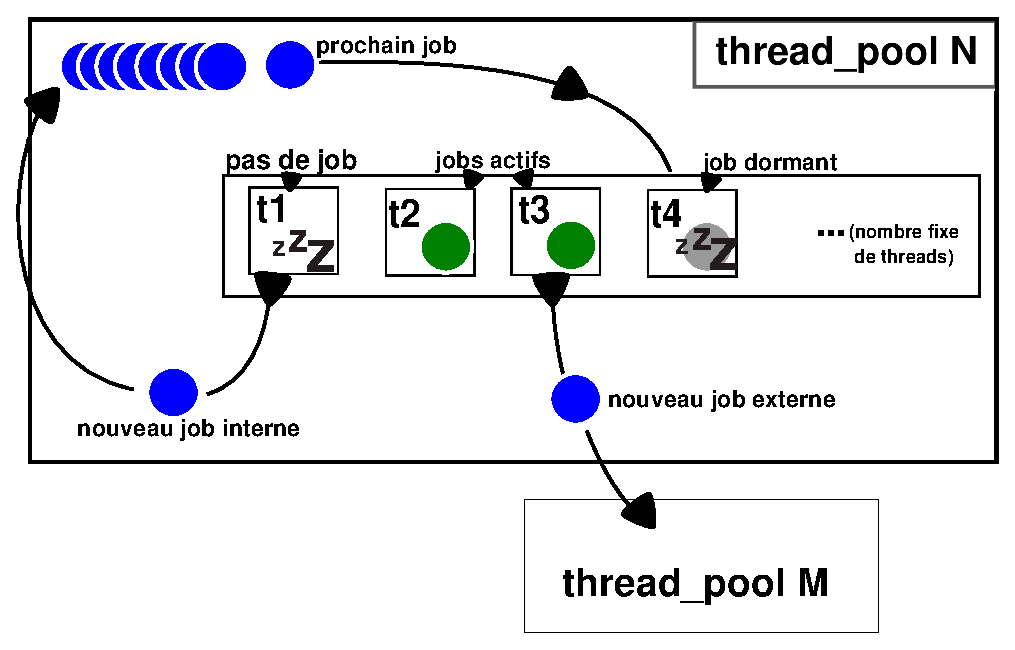
\includegraphics[scale=0.5]{thread_pool.eps}
    \caption{Fonctionnement d'un pool de threads.}
    \label{fonctionnement}
\end{figure}
\end{center}


